\chapter{Conclusions and further discussion}

\section{Summary of results}

\subsection{Restatement of project aims}

The main aim was to learn jointly aligned probabilistic embeddings, represented by multidimensional Gaussian distributions with diagonal covariance, for concepts in the Open Images and AudioSet domains. Alignment and embedding learning were to happen concurrently. Independently learned probabilistic embeddings (training each domain separately) were also run as a baseline. The quality of these embeddings was examined by comparing the Spearman correlation of their pairwise similarities with three different human-curated similarity measures (only two for AudioSet due to lack of data)- MTURK-771 \cite{mturk771}, WordNet \cite{WordNet}, and ILSVRC \cite{RoadsLoveCVPR}. Ideally, the aligned embeddings would be of higher quality (more similar with human judgement) than the independently learned embeddings. 

\subsection{Independently learned probabilistic embeddings}

\subsubsection{Clustering}
The means of the probabilistic embeddings represent sensible clusters when viewed through scatter plots of t-SNE dimensionality reduction down to 2 dimensions. Qualitatively, items in the concept hierarchy that represent more abstract concepts from the point of view of the hierarchy (``Cat", ``Dog") have nearest neighbours that are not very well clustered. Items that are more specific (``Domestic short-haired cat")  have nearest neighbours that are more sensible. Examples of these phenomena are shown in Tables \ref{table:cat} and \ref{table:subclasscat}. 

\subsubsection{Statistics}
The variances of the independently learned embeddings,  when expressed as entropies, correlate negatively with co-occurrence frequency (Table \ref{table:entropiescorr}). Concepts which occur less frequently in the input data have a higher variance. This is an expected result- there is more uncertainty about concepts that occur less frequently. 

\subsection{Semi-supervised learning of aligned embeddings}

\subsubsection{Alignment}
Our algorithm successfully learned jointly aligned embeddings from two modalities, Open Images containing 19996 concepts and AudioSet containing 526 concepts, with an intersection of 230 concepts. Embeddings for both domains were learned simultaneously along with alignment, with no post-processing necessary to achieve alignment. The 230 intersecting concepts were used as semi-supervised input into the algorithm by tying their mapped values together during training as part of the loss function. 

Alignment accuracy, as measured by the number of concepts in one domain whose nearest neighbour in the mapped domain was the true corresponding concept in the other domain (as described in Section \ref{section:alignmentdef}), of more than 95\% was obtained between the two domains, for the intersecting concepts. However, convergence to this level of accuracy while still maintaining sensible clustering (avoiding the degenerate case displayed in Figure \ref{fig:dysfunctional_clusters}) required some tuning of the model parameters, as described in Section \ref{section:otherparameters}
    
The criterion for saving the embeddings was when the mean alignment accuracy (of both OpenImages and AudioSet embeddings) was the highest. Knowing that the independently learned probabilistic embeddings for AudioSet required more epochs of training to converge than the similar case of Open Images, it is possible that the point of greatest alignment accuracy for AudioSet is at a different epoch than for Open Images, but that training to achieve this would cause a decrease in accuracy for Open Images. 

\newpage
\subsubsection{Embedding quality}
As a baseline, the aligned embeddings also displayed sensible semantic clustering (Figures \ref{fig:openimagesaligned} and \ref{fig:audiosetaligned}). \textbf{Embedding quality as measured by Spearman correlation of embedding pair similarity and WordNet similarity measures was greater for the aligned Open Images embeddings than the independently learned Open Images embeddings.} When measuring by Spearman correlation of embedding pair similarity and ILSVRC / MTURK-771 datasets, embedding quality for the aligned Open Images was decreased compared to the independently learned embeddings.     

\textbf{For AudioSet embeddings, embedding quality as judged by the WordNet and ILSVRC metrics was greater for aligned than independently learned embeddings.} A comparison with MTURK-771 was not run for AudioSet due to lack of data (only 3 pairs overlapped).  

Including the empirical MMD statistic in the loss function increased alignment accuracy for both domains, but had varying effects on other measures of embedding quality. The MMD statistic increased embedding quality as measured by the Spearman correlation with WordNet similarity for the Open Images domain. For AudioSet and for Open Images compared with MTURK-771 and enhanced ILSVRC, MMD was either ineffective or decreased embedding quality. 

The entropy of the aligned embeddings became decorrelated with the frequency of occurrence of each concept, compared to independently learned embeddings. The stability of aligned embeddings is also lower than that of independently learned embeddings, in that the top 5 nearest neighbours of concepts are more different over different runs.

\textbf{We conclude that there is some evidence that aligned embeddings are of higher quality than independently learned embeddings, and therefore that learning from multiple modalities simultaneously helps generalise to better representations for both modalities.} The results of comparing embedding quality based on WordNet lexical database similarity scores indicated that aligned embeddings are more closely correlated with human judgement. However, the comparisons with the two datasets using direct human-collected scores (MTURK-771 and enhanced ILSVRC) gave mixed results. Given that the latter two datasets are much smaller in comparison to WordNet, this bears further investigation. 

%\subsection{Computational performance}

%When run using one GeForce RTX 2080 GPU, 150 epochs took about half an hour where most of the time taken was actually saving the model to disk when the mean epoch accuracy was greater than the previous epoch's accuracy (the actual model runtime was much less). 

%The most significant bottleneck in the process was actually creating the co-occurrence matrix for OpenImages, as there are close to 20000 concepts in the dataset, and this information was contained in a 57 million line text file (this process took 2.5 hours). However this only needed to be done once.

\section{Directions for future research}

\subsection{Controlling for different domain distributions}
Alignment of embeddings from two different domains requires synchronising two distributions that have very different statistics. We already see that the sizes of the datasets are very unbalanced, and there is little overlap of concepts. To control for this, we could try splitting one dataset into 2 parts with a defined amount of overlap (for example, 2 subsets of 10000 concepts from Open Images, with an intersection of 2000 concepts) and trying to align those two subsets. This should allow us to learn about the alignment problem independently from the influence of the statistics of the different domains. We already encountered one issue which was that the GloVe loss needed to be scaled to achieve good convergence from the point of view of alignment accuracy. 

\subsection{Model parameters}

As the problem and full loss function (Equation \ref{eq:fulllossfunction}) are complex and contain many terms, they are likely to be very sensitive to initial conditions and choice of optimiser and learning rate. Cross-validation could be used to investigate better choices. 

The use of alignment accuracy itself as a measure of convergence could be reconsidered for further experiments. We already see that with the use of MMD, alignment accuracy could increase but with a corresponding decrease in embedding quality; perhaps there is a way of including some measure of embedding quality in the stopping criteria or loss function.  

\subsection{Embedding dimensionality}
Appropriate dimensionality of the embeddings for both domains should be investigated. As mentioned earlier, this number was chosen heuristically (keeping the ratio of concepts relative to the dimension the same as that of the original GloVe word embedding problem \cite{pennington2014glove}). Further studies should involve cross-validation to investigate appropriate dimensionality, which may not be the same for both domains. Tests with the independent embeddings showed that if dimensionality was too high (the example was dimension of 30 used for AudioSet embeddings), the resulting embeddings did not demonstrate good clustering as visualised through t-SNE. 

\subsection{Hierarchy of concepts}
The highly non-overlapping concept sets mean that there are many concepts present in Open Images that are not specifically present in AudioSet. However, the Open Images concepts are actually at many levels of hierarchy. For example, there are different types of cat and different types of dog. Thus many of these may actually map to a single concept in AudioSet, and there is no provision for this at the moment. 

Incorporating some form of hierarchy may lead to better results. This hierarchy may represented implicitly or explicitly.   We saw that the nearest neighbours by distance to concepts that are higher up in the class hierarchy were less related than the nearest neighbours of concepts that are closer to the leaf nodes (Tables \ref{table:cat} and \ref{table:subclasscat}), and this is possibly because Euclidean distance does not represent hierarchy well \cite{NNAnalysisPsychologicalSpaces}. Poincar{\'{e}} embeddings \cite{PoincareEmbeddings} use distance measures in non-Euclidean space (hyperbolic in this case) to allow hierarchical concepts to be represented implicitly.

Some explicit hierarchy information is available associated with the datasets, which we do not currently use. A partial such tree is shown in the figure below:

\begin{figure}[H]
\label{fig:tree}
    \centering
    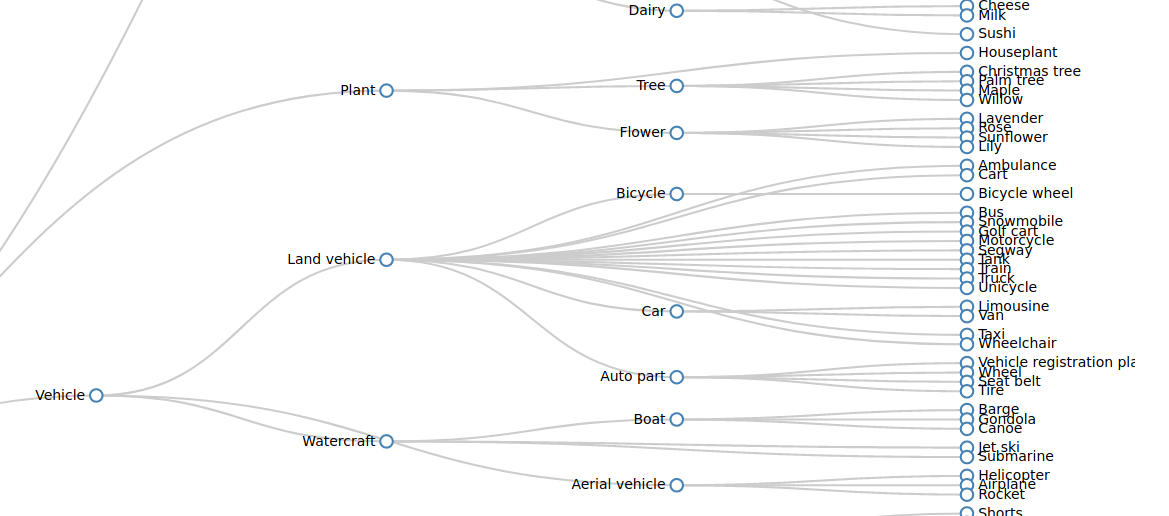
\includegraphics[width=0.75\textwidth]{images/conclusions/tree.png}
    \caption{
        Tree structure showing part of the Open Images concept hierarchy. A similar structure exists for AudioSet.
    }
\end{figure}

From the t-SNE visuations of the independent embeddings as seen in Figures \ref{fig:openimages1} and \ref{fig:openimages2}, it is clear that concept classes form clusters. We saw that the differences in arrangement of these clusters over different runs are not a simple spatial transformation (combining rotations, translations and stretching only). One obvious modification to the algorithm might be to align the parent concept classes for example ``Cat" and ``Dog" as a first pass, and then to align the subclasses around these anchor concepts. This process of multiple alignment passes has been used in \cite{UnsupervisedAlignmentWP} to perform alignment of cross-lingual word embeddings for bilingual lexicon induction. 

There are many aural concepts that obviously will not have a visual representation, so this is yet another limitation of using these particular two modalities. Better results may perhaps be obtained by trying to align embeddings derived from Open Images and text, but then we would have to solve the following practical problems:

\begin{itemize}
    \item How to resolve words to the Open Images namespace; one such possibility was used when running similarity comparisons with WordNet, described in the previous chapter. There is no sense information in the Open Images namespace, though it is noticeable that most of the categories are nouns.  
    \item How to extract not just single words but phrases from the text, for example, ``domestic short-haired cat". Computationally this can pose a problem as the vocabulary size of text corpora is already large, and now we would have to maintain n-grams as well to try and capture entire phrases. 
\end{itemize}


\subsection{Unsupervised learning of aligned embeddings}

The experiments in this project lead to the ultimate goal of learning aligned embeddings in an unsupervised way, in keeping with the desire to emulate human learning. In this situation the concept universes for both domains are known, as are the items in the intersection. However the specific embeddings in the intersection in each domain would not be directly mapped in the losses during learning. Aggregate statistics of the domain intersection might be used, such as the MMD. 

Preliminary work was unable to produce accuracies greater than 1\% for unsupervised alignment, using the same model configuration as the semi-supervised case, only excluding the distance loss that related $||f(x) - y||$ and $||g(y) - x||$. It is possible that including some measure of graph-based similarity between the embeddings may increase convergence. The Friedman-Rafsky statistic described in \cite{torchtwosample} was tried, but there was no perceptible convergence.

Further preliminary work also tested the Manifold Alignment GAN \cite{magan} and the Wasserstein GAN \cite{WassersteinGAN}, using the configurations described in the respective papers, with the full loss function as in  equation \ref{eq:fulllossfunction} used as the generator loss. Neither of these produced any feasible alignment. Mode collapse (all concepts mapping to the same embedding) was at first an issue, but even with using the minibatch discrimination technique \cite{ImprovedTechniquesTrainingGANS} to remove this possibility, no feasible alignment was found. The discriminator loss was asymptotically minimal, indicating that the discriminators were not able to tell the mapped values from the real values, but there was still no alignment. It is possible that there are simply no manifolds to align for the number of dimensions we have chosen (6) for our embeddings. 

It is known that GANs do well on problems where the input data fall into specific discernible classes, and our dataset does not have this characteristic. Though there are discernible clusters, they are indistinct as befits a human taxonomy of concepts rather than visual representations of 10 digits, or works by different artists. Given this constraint, it is reasonable that a naive GAN might not work. In particular, there were different numbers of elements in the source and target domains; neither the MAGAN nor Wasserstein GAN were tested in this situation. Additionally, \cite{ImprovedTechniquesTrainingGANS} found that the ILSVRC2012 dataset with 1000 categories was a challenge for their GAN because of the large number of classes, which is already fewer than the 19996 in our Open Images dataset. Much existing GAN research has been done on generating images matching certain criteria, for which input data is plentiful (some input sets number in the millions). In addition to having a very large number of classes, we also only have one example of each, so it should be considerably more difficult to learn this distribution with a GAN. 

Lastly, previous experiments in the Love Lab \cite{AraoThesis} found that the Wasserstein (Equation \ref{eq:wasserstein}) and Sinkhorn (a regularised version of the Wasserstein) distances could be used as loss functions for unsupervised alignment of concept embeddings, but these experiments were run on synthetic data generated from Gaussian mixture models. Therefore it is conceivable that the Wasserstein and Sinkhorn distances could serve as loss functions for alignment of embeddings constructed from real data, with appropriate configuration. 